\documentclass[a4paper, 11pt]{article}

\usepackage{xcolor}
\input{/home/aroquemaurel/cours/templates/templates/couleurs.tex}
\usepackage{lmodern}
\usepackage[utf8]{inputenc}
\usepackage[T1]{fontenc} \usepackage[francais]{babel}
\usepackage[top=1.7cm, bottom=1.7cm, left=2.5cm, right=2.5cm]{geometry}
\usepackage{verbatim}
\usepackage{tikz} %Vectoriel
\usepackage{pgfplots}
\usepackage{listings}
\usepackage{fancyhdr}
\usepackage{multido}
\usepackage{amssymb}
\usepackage{multicol}
\usepackage{float}
\usepackage[urlbordercolor={1 1 1}, linkbordercolor={1 1 1}, linkcolor=vert1, urlcolor=bleu, colorlinks=true]{hyperref}

\newcommand{\titre}{Gestion de sous-titres dans un flux vidéo}
\newcommand{\numero}{2}
\newcommand{\typeDoc}{DM}
\newcommand{\module}{Outils Informatiques pour le Multimédia}
\newcommand{\sigle}{OIM}
\newcommand{\semestre}{7}
\newcommand{\auteur}{Antoine de \bsc{Roquemaurel} (G1.1)}

\input{/home/aroquemaurel/cours/templates/templates/classroomsTemplates/l3/tddm.tex}
\input{/home/aroquemaurel/cours/templates/templates/listings.tex} %prise en charge du langage C 
\input{/home/aroquemaurel/cours/templates/templates/classroomsTemplates/l3/remarquesExempleAttention.tex}
\input{/home/aroquemaurel/cours/templates/templates/polices.tex}
\input{/home/aroquemaurel/cours/templates/templates/affichageChapitre.tex}
\makeatother

\begin{document}
	\maketitle
	\section{Partie I : en ligne de commande}
	\subsection{Les formats OGV, Vorbis et Theora}
	Avant de pouvoir définir ces trois formats, il parait important de définir le projet OGG.

	OGG est un projet libre issue de la fondation Xiph.org, ce projet à pour but de fournir des formats audio et vidéo qui soient libre. Plusieurs formats de
	fichiers ont ainsi vu le jour : \texttt{.oga} pour les fichiers audio, \texttt{.ogv} pour les fichiers vidéos et \texttt{.ogx} pour les applications.
	
	Les formats que je vais définir ci-dessous sont tous issues du projet OGG.
	\begin{description}
		\item[OGV] est le format issue du projet OGG permettant de lire des vidéos compressée tout en gardant une excellente qualité.
		\item[Vorbis] est un format de compression/décompression audio libre, il peut faire concurrence au format propriétaire \texttt{.mp3}, cependant celui-ci est
			moins connu et n'est supporté que par peu de lecteur audio bien qu'il ait de meilleurs performance que son concurrent.
		\item[Theora] est un format de compression/décompression vidéo libre, il est souvent couplé à \textit{vorbis} pour l'audio, il est ainsi possible de lire une
			vidéo avec le son. Il est soutenu par de nombreux logiciels libres tel que Firefox ou les distributions GNU/Linux. 
	\end{description}
	\subsection{Lire une vidéo}
	\subsubsection{Lire un fichier audio}
	\begin{lstlisting}[numbers=none,language=sh, caption=Lire un fichier audio -- Uniquement pour les fichier \texttt{.oga}]
gst-launch filesrc location=music.oga ! oggdemux ! vorbisdec ! audioconvert ! alsasink
	\end{lstlisting}
	\begin{lstlisting}[numbers=none,language=sh, caption=Lire un fichier audio -- Pour tous les formats audio]
gst-launch filesrc location=music.oga ! decodebin ! audioresample ! autoaudiosink
	\end{lstlisting}
	\subsubsection{Lire une vidéo avec le son}
	\begin{lstlisting}[numbers=none,language=sh, caption=Lire une vidéo -- Uniquement pour les fichier \texttt{.ogv}]
gst-launch filesrc location=video.ogv ! oggdemux ! theoradec ! ffmpegcolorspace ! autovideosink
	\end{lstlisting}
	\begin{lstlisting}[numbers=none,language=sh, caption=Lire une vidéo -- Pour tous les formats audio-vidéos]
gst-launch filesrc location=video.ogv ! decodebin ! autovideosink
	\end{lstlisting}
	\begin{remarque}
		Le plugin \textit{decodebin} permet à \textit{GStreamer} de détecter lui même la nature du conteneur et du codec à utiliser. Ainsi, nous pouvons lire une multitude de
		formats différents en utilisant celui-ci.

		Dans le projet, seul \textit{oggdemux} et \textit{theoradec} ont été utilisés.
	\end{remarque}
	\subsubsection{Lire une vidéo en remplaçant l'audio}
	\begin{lstlisting}[language=sh, caption=Lire une vidéo avec le son de source différente]
gst-launch filesrc location=video.ogv ! decodebin ! autovideosink filesrc location=music.oga ! decodebin ! autoaudiosink
	\end{lstlisting}
	\subsection{Lire une vidéo avec des sous-titres}
	\begin{lstlisting}[language=Bash, caption=Lire une vidéo avec des sous-titres \texttt{.srt}]	
gst-launch filesrc location=video.ogv ! oggdemux name=demux \ 
	filesrc location=video.srt ! subparse ! overlay. \
	demux. ! queue ! vorbisdec ! audioconvert !  autoaudiosink \
	demux. ! queue ! theoradec ! ffmpegcolorspace ! \
	subtitleoverlay name=overlay ! autovideosink
\end{lstlisting}
	\subsection{Enregistrer une vidéo avec les sous-titres incrustés et un son externe}
	\begin{lstlisting}[language=Sh, caption=Enregistrer une vidéo avec l'audio \texttt{music.oga}\, l'image \texttt{video.ogv} et les sous-titres]
gst-launch filesrc location=video.ogv ! oggdemux name=demux \
filesrc location=music.oga \
! queue ! oggdemux ! vorbisdec ! audioconvert ! vorbisenc ! mux. demux. \
! queue ! theoradec !  subtitleoverlay name=sub !  theoraenc ! \
mux. filesrc location =./video.srt !  subparse ! sub. oggmux name=mux ! \
filesink location=videoQ4.ogv
	\end{lstlisting}
	\section{Partie II : en programmation C++}
	Pour cette partie, j'ai choisi de développer l'application en C++, comme proposé dans le sujet. En effet, j'affectionne tout particulièrement ce langage en
	raison de sa rapidité, de sa souplesse tout en restant extrêmement puissant et en utilisant le paradigme orienté objet.

	L'application que j'ai développé ne permet de ne lire que des fichier au format \texttt{OGV} ou \texttt{Theora}, en raison des chaînes de traitement que j'ai
	choisi d'utiliser. Il aurait été éventuellement possible d'utiliser \texttt{decodebin} afin d'être ouvert au maximum de formats possible, cependant celui-ci
	rendait l'utilisation des sous-titres plus complexe.

	Une autre solution permettant de mener ce projet à bien plus simplement aurait été l'utilisation de \texttt{playbin2}, cependant celui-ci n'étant pas
	autorisé pour réaliser ce sujet, je me suis restreint au format \texttt{OGV}.

	\subsection{Question 5}
	\begin{lstlisting}[language=sh]
 aroquemaurel@Luffy ~/projets/cpp/videos-reader <master> ./lecteurvideo video.ogv 
	\end{lstlisting}
	\begin{figure}[H]
		\centering
		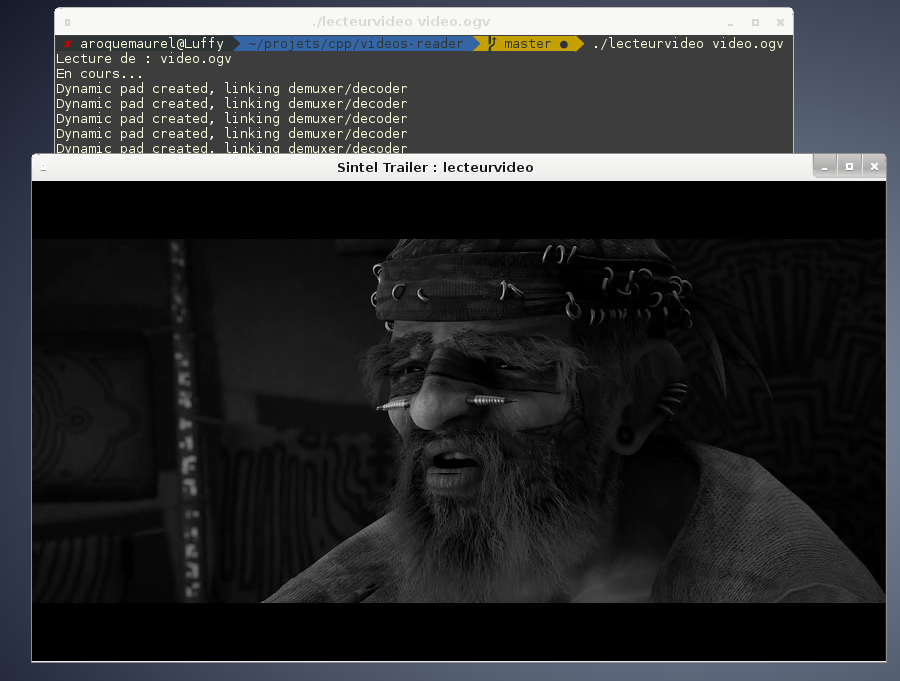
\includegraphics[width=17cm]{img/1.png}
		\caption{Lecteur vidéo sans interface}
	\end{figure}
	Comme prévu dans le TP5, la vidéo est grisé est le son est réduit de 50\%. 

	J'ai cependant modifié légèrement le code fournit, dorénavant, j'ai créé une classe permettant de fournir des méthodes pour tous les \texttt{GstElement}.
	L'interface de cette classe me permet d'éviter d'avoir des dizaines de variables déclarés\footnote{Ceci grâce à une \texttt{std::map}}, de vérifier que tout a été alloué correctement et de tout ajouter
	automatiquement au pipeline, ceux en un minimum de lignes.
	
	\begin{lstlisting}[language=C++, caption=Interface de gestion des commandes GStreamer]
class GStreamerCommands {
public:
	GStreamerCommands(void);
	~GStreamerCommands(void);

	void setElement(std::string nameElement, const std::string nameArg, const std::string valuePropertie);
	void setElement(std::string nameElement, const std::string nameArg, const double valuePropertie);
	void setElement(std::string nameElement, const std::string nameArg, const bool valuePropertie);
	GstElement *getElement(std::string s);
	void addElement(std::string name, std::string value);

	void checkAllElements(void);
	void addAllElements(void);
	GstElement *getPipeline(void) const;
	void setPipeline(GstElement *getPipeline);
};
	\end{lstlisting}
	\subsection{Affichage des sous-titres}
	Afin d'afficher des sous-titres, j'ai utilisé la ligne de commande suivante : 
	\begin{lstlisting}[language=sh]
		gst-launch filesrc location=video.ogv ! oggdemux name=demux \
		filesrc location=video.srt ! subparse ! overlay. \
		demux. ! queue ! vorbisdec ! audioconvert ! autoaudiosink \
		demux. ! queue ! theoradec ! ffmpegcolorspace ! subtitleoverlay name=overlay ! autovideosink;
	\end{lstlisting}

	J'ai donc ajouté les éléments suivants, et ensuite effectué le linkage correctement : 
	\begin{lstlisting}[language=C++]
		// Add all srt elements
		_commands->addElement ("subOverlay",  "subtitleoverlay");
		_commands->addElement ("subSource",   "filesrc");
		_commands->addElement ("subParse",    "subparse");

		// Linkage
		gst_element_link_many (_commands->getElement("videoQueue"), _commands->getElement("videoDecoder"),
		_commands->getElement("videoConv"), _commands->getElement("subOverlay"),
		_commands->getElement("videosink"), NULL);
		gst_element_link_many (_commands->getElement("audioQueue"), _commands->getElement("audioDecoder"),
		_commands->getElement("audioConv"), _commands->getElement("audiosink"), NULL);
		g_signal_connect (_commands->getElement("demuxer"), "pad-added", G_CALLBACK (on_pad_added), _commands->getElement("audioQueue"));
		g_signal_connect (_commands->getElement("demuxer"), "pad-added", G_CALLBACK (on_pad_added), _commands->getElement("videoQueue"));
	\end{lstlisting}

	\begin{figure}[H]
		\centering
		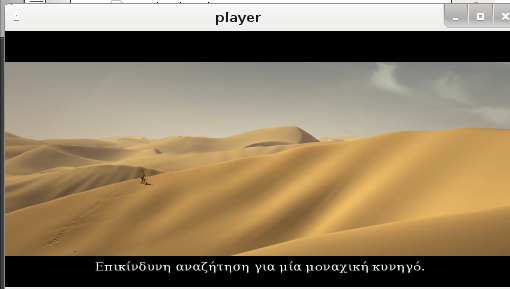
\includegraphics[width=14cm]{img/2.png}
		\caption{Lecteur vidéo avec sous-titres sans interface}
	\end{figure}
	\subsection{Interface GTK}
	Mon projet à été pensé en respectant le pattern \texttt{M VC}, Modèle Vue-Contrôleur.

	\begin{description}
		\item[Modèle] Le backend du logiciel, l'appel aux méthodes gstreamer.
		\item[Vue] Ce qui a attrait à l'apparence et l'interaction, tout est présent dans la classe Ui
		\item[Contrôleur] Qui se charge de faire le lien entre le modèle et la vue. Ici il est lié à la vue, on peut considérer que les méthodes de callback sont
			le contrôleur.
	\end{description}

	\begin{remarque}
		GTK à été conçu pour le C et non pour le C++, ainsi cette bibliothèque fonctionne principalement avec un système de callbacks et de foncteur, chose
		difficilement réalisable dans une classe C++. J'ai donc une classe \texttt{Ui} possédant une majorité de méthodes statiques. 

		Il aurait été plus élégant d'utiliser la bibliothèque \textit{Gtkmm}, bibliothèque GTK pensée pour le C++ permettant d'avoir toute la puissance du
		paradigme objet. Cependant, celle-ci n'étant pas installée en salle de TP, je n'ai pas pu m'en servir.
	\end{remarque}

	% TODO FIGURE
	\begin{figure}[H]
		\centering
		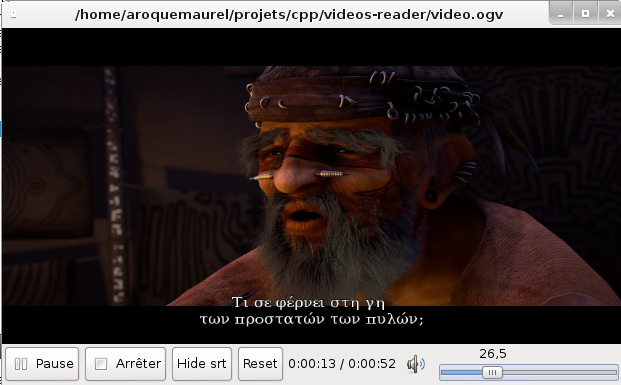
\includegraphics[width=15cm]{img/3.png}
		\caption{Interface du lecteur multimédia développé}
	\end{figure}
	\begin{remarque}
		Les images présents dans les boutons sont des images obtenus du gestionnaire de bureau, ici Mate, il se peut que chez vous ceux-ci s'affichent
		différemment, ou ne s'affiche pas du tout. 

		Cet affichage permet d'avoir un système d'exploitation uniformisé, GTK possède une multitude de boutons prédéfinis, pour cela il suffit de créer un
		bouton comme suit.
		\begin{lstlisting}[language=C, numbers=none,linewidth=400px ]
			stop_button = gtk_button_new_from_stock (GTK_STOCK_MEDIA_STOP);
		\end{lstlisting}
	\end{remarque}

	\subsection{Fonctionnalités ajoutées au lecteur}
	Le lecteur précédent étant assez basique, plusieurs fonctionnalités ont été ajoutés au lecteur audio-vidéo afin de gagner en confort : 
	\begin{itemize}
		\item Une barre << slider >> permettant d'observer l'avancement du programme et de contrôler la vidéo
		\item Un label affichant la durée de la vidéo, et le
			temps actuel parcouru.\footnote{Au format hh:mm:ss, à l'aide de la macro \texttt{GST\_TIME\_FORMAT}}
		\item Une possibilité de mettre la vidéo en plein écran, à l'aide de la touche << F >> ou << F11 >>.
		\item Gestion du son via le bouton de son. Celui-ci va de 0 à 2 fois le son original de la vidéo.
	\end{itemize}

	J'ai également mis en place des raccourcies à l'aide du clavier afin que l'utilisateur gagne au maximum du temps : 

	\begin{tabular}{c|p{10cm}}
		\textbf{Touche du clavier} & \textbf{Action}\\
		\hline
		F ou F11& Met la vidéo en Met la vidéo en plein écran\\
		\hline
		Barre d'espace ou P&Pause ou play en fonction de l'état courant de la vidéo\\
		\hline
		S&Affiche ou cache les sous-titres en fonction de l'état actuel des sous-titres\\
		\hline
		R&Redémarre la vidéo\\
		\hline
		Q&Quitte le lecteur vidéo\\
		\hline
		<< Backspace >> / Retour arrière &Stop la lecture de la vidéo \\
		\hline
		Flèches gauche et droite&Recule ou avance respectivement dans la vidéo\\
		\hline
		Flèche haut et bas & Augmente ou diminue le volume sonore\\
		\hline
	\end{tabular}
	\subsection{Activer ou désactiver les sous-titres}
	L'utilisateur peut activer ou non les sous-titres à l'aide du bouton situé en bas de l'interface. 

	Afin de pouvoir afficher ou non les sous-titres, il m'a suffit d'utiliser l'argument \texttt{silent} de \texttt{subtitleoverlay}.
	\begin{lstlisting}[language=C++, caption=Affichage ou non des sous-titres]
		// Désactive les sous-titres
		g_object_set (G_OBJECT (_commands->getElement("subOverlay")), "silent", false, NULL); 
		// Active les sous-titres
		g_object_set (G_OBJECT (_commands->getElement("subOverlay")), "silent", true, NULL); 

		// Ou avec mon interface
		_commands->setElement("subOverlay", "silent", false);

	\end{lstlisting}
	\appendix
	\lstlistoflistings
	\listoffigures
	\end{document}
